\begin{question}
\noindent Triangle $S$ has vertices at $A(1,1)$, $B(4,1)$ and $C(1,3)$.

\noindent Triangle $S$ is rotated $90^\circ$ clockwise about the origin $O$ to give triangle $S'$.

\begin{center}
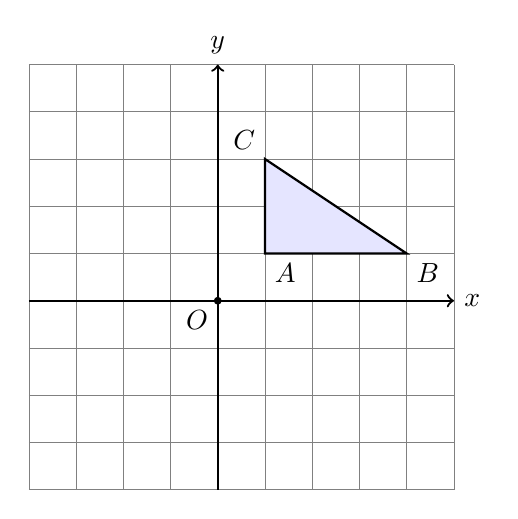
\begin{tikzpicture}[scale=0.6]
    \draw[step=1, gray, very thin] (-4,-4) grid (5,5);
    \draw[thick, ->] (-4,0) -- (5,0) node[right]{$x$};
    \draw[thick, ->] (0,-4) -- (0,5) node[above]{$y$};

    \draw[thick, fill=blue!10] (1,1) -- (4,1) -- (1,3) -- cycle;
    \node[below right] at (1,1) {$A$};
    \node[below right] at (4,1) {$B$};
    \node[above left] at (1,3) {$C$};

    \node[below left] at (0,0) {$O$};
    \filldraw (0,0) circle (2pt);
\end{tikzpicture}
\end{center}

\noindent On the grid, draw triangle $S'$, the image of triangle $S$ after a rotation of $90^\circ$ clockwise about the origin $O$.

\vspace{4cm}

\begin{flushright}
    \answerplain{3}
\end{flushright}
\end{question}